\chapter{Identification of Transfer Function of a Single Board Heater System through Step Response Experiment}\label{chap1}
The aim of this experiment is to perform step test on a Single Board Heater System and to identify system transfer 
function using step response data. The target group is anyone who has basic knowledge of control engineering.

\begin{figure}
\centering
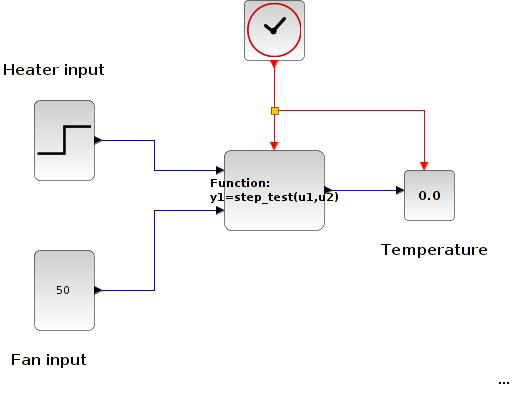
\includegraphics[width=\linewidth]{Step-test_manual/step_xcos.jpg}
\caption{Xcos for this experiment}
\label{xcos_st}
\end{figure}

\begin{figure}
\centering
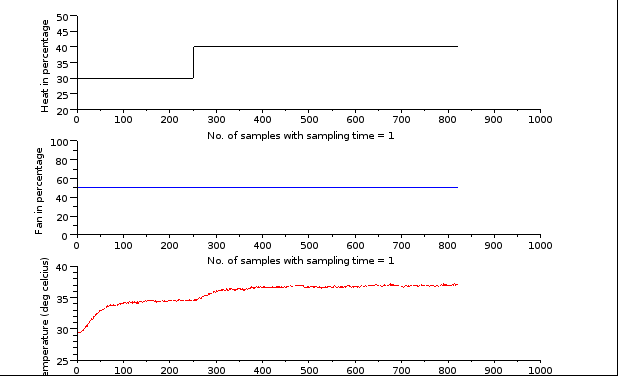
\includegraphics[width=\linewidth]{Step-test_manual/ste-test.png}
\caption{Graph shows heater current, fan speed and output temperature}
\label{fig:scope_st}
\end{figure}

We have used Scilab and Xcos as an interface for sending and receiving data. 
Xcos diagram is shown in figure \ref{xcos_st}. Heater current and fan speed are the two inputs for this system. 
They are given in percentage of maximum. These inputs can be varied by setting the properties of the input block's properties 
in Xcos. The plots of their amplitude versus number of collected samples are also available on the scope windows. 
The output temperature profile, as read by the sensor, is also plotted. The data acquired in the process is stored on the 
local drive and is available to the user for further calculations.

 In the {\tt step\_test.xcos} file, open the heater block's parameters to apply a step change of say 10 percent to the heater at operating point of 30 percent of heater after 250 seconds. The block parameters of the step input block will have {\tt Step time = 250}, {\tt Initial value = 30} and {\tt Final value = 40}. 
Keep the fan input constant at 50 percent. Start the experiment and let it continue until you see the temperature 
reach the steady state. 

\begin{table}
\begin{verbatim}
 1.0    30.0    50.0    29.3   1412400132192.0
 2.0    30.0    50.0    29.5   1412400133044.0
.
.
820.0    40.0     50.0    37.0   1412400950197.0
821.0    40.0     50.0    37.2   1412400951202.0
\end{verbatim}
\caption{Step data obtained after performing local Step Test}
\label{stepdata}
\end{table}

The step test data file will be saved in {\tt Step\_test} folder. The name of the file will be the date and time at which the experiment was conducted. A sample data file is provided in the same folder. The sample data file is named as {\tt step-data-local.txt} and {\tt step-data-virtual.txt}. Refer to the one depending on wheather you are performing a local or a virtual experiment. Referring to the data file thus obtained as shown in table \ref{stepdata}, the first column in this table denotes samples. The second column in this table denotes heater in percentage. It starts at 30 and increases with a step size of 10 units. The third column denotes the fan in percentage. It has been held constant at 50 percent. The fourth column refers to the value of temperature. The fifth column denotes time stamp. The virtual data file will havel four time stamp columns apart from first 3 columns. These four time stamp columns are client departure, server arrival, server departure and client arrival. These can be used for advanced control algorithms. These additional time stamps exist in virtual mode because of the presense of network delay.
\section{Conducting Step Test on SBHS locally}
The detailed procedure to perform a local experiment is explained in Chapter\ref{sercomm}. A summary of the same is provided in section \ref{local-summary} It is exactly the same for this section. The response is as shown in figure \ref{fig:scope_st}. The output data file is as shown in Table \ref{stepdata}
\section{Conducting Step Test on SBHS, virtually}
The detailed procedure to perform a local experiment is explained in Chapter\ref{virtual}. A summary of the same is provided in section \ref{vlabsexpt} It is exactly the same for this section. The virtual experiment response is shown in figure \ref{step-virtual}. The corresponding data file is shown in table \ref{stepdata}. The time stamps shown are cut short for better viewing. This data file can be found in {\tt StepTest} folder for virtual experiments. The name of this file is {\tt step-data-virtual.txt}.


\begin{figure}
\centering
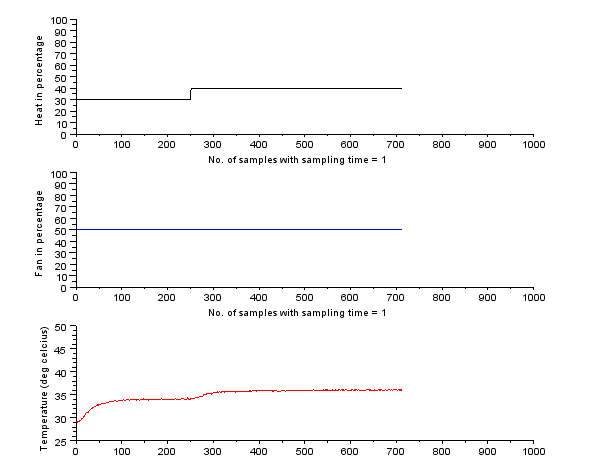
\includegraphics[width=\linewidth]{Step-test_manual/step-virtual.png}
\caption{Step test Virtual experiment response}
\label{step-virtual}
\end{figure}


\begin{table}
\begin{verbatim}
 0 0 100 29.30 14...8080 14...8955 14...8993 14...8158 0.10000E+01
1 30 50 29.00 14...9364 14...0246 14...0263 14...9442 0.10000E+01
.
.
711 40 50 36.20 14...9375 14...0280 14...0297 14...9437 0.71100E+03
712 40 50 36.10 14...0370 14...2673 14...2691 14...1834 0.71200E+03
\end{verbatim}
\caption{Step data obtained after performing virtual Step Test}
\label{stepdata}
\end{table}

\section{Identifying First Order and Second Order Transfer Functions}
In this section we shall determine the first and second order transer function model using the data obtained after performing step test experiment. Please note that this procedure is common for data obtained using both local and virtual experiments.


\subsection{Determination of First Order Transfer Function}
Identification of the transfer function of a system is important as it helps us to 
represent the physical system mathematically. Once the transfer function is obtained, one can acquire 
the response of the system for various inputs without actually applying them to the system.

Consider the standard first order transfer function given below
\begin{align}
G(s) &= \frac{ C(s)}{ R(s)}\label{1}\\
G(s)&=\frac 1{\tau s+1}\label{std_fo}                           
\intertext{Rewriting the equation, we get}
C(s)  &= \frac {R(s)}{\tau s + 1}\label{rw_std_fo}
\intertext{A step is given as input to the first order system. The Laplace 
transform of a step function is$ \frac {1}{s}$. Hence, substituting $ R(s) = \frac {1}{s}$ in equation \ref{rw_std_fo}, 
we obtain}
C(s) & = \frac 1{\tau s + 1}\frac 1{s}\label{sub_rs}\\
\intertext{Solving $C(s)$ using partial fraction expansion, we get}
C(s) &= \frac1{s} - \frac {1}{s + \frac1 \tau}\label{pf}
\intertext{Taking the Inverse Laplace transform of equation \ref{pf}, we get}
c(t)&= 1 - e^{\frac {-t}\tau }\label{lti} 
\end{align}
From the above equation it is clear that for t=0, the value of c(t) is zero. For t= $\infty$, c(t) 
approaches unity. Also, as the value of \textquoteleft t \textquoteright  becomes equal to $\tau$, 
the value of c(t) becomes 0.632. $\tau$ is called the time constant and represents the speed of 
response of the system. But it should be noted that, smaller the time constant- faster the system response.
By getting the value of $\tau$, one can identify the transfer function of the system. 

Consider the system to be first order. We try to fit a first order transfer function of the form
\begin{align}       
G(s) &= \frac K{\tau s + 1}\label{7}
\intertext{to the Single Board Heater System. Because the transfer function approach uses deviation 
variables, $ G(s)$ denotes the Laplace transform of the gain of the system between the change in heater 
current and the change in the system temperature. Let the change in the heater current be denoted by $\Delta u$.  
We denote both the time domain and the Laplace transform variable by the same lower case variable. Let the change 
in temperature be denoted by $y$. Let the current change by a step of size $u$. Then, we obtain the following 
relation between the current and the temperature.} 
y(s) &= G(s)u(s)\\ 
y(s)&= \frac K{\tau s + 1}{\frac  {\Delta u}{{s}}}
\intertext {Note that $\Delta$ u is the height of the step and hence is a constant. On inversion, we obtain}
y(s)&= K[1 - e^{\frac{-t}\tau}]\Delta u
\end{align}
\subsection{Procedure}
\begin{enumerate}
\item Download the Analysis folder from the sbhs website. It will be available under {\tt downloads} section. Download the file for {\tt SBHS Analysis Code (local \& virtual)}. The name of the file is {\tt scilab\_codes\_analysis}. The download will be in zip format. Extrat the downloaded zip file. You will get a folder {\tt scilab\_codes\_analysis}. 
\item Open the {\tt scilab\_codes\_analysis} folder and then locate and open the folder {\tt Step\_Analysis}.
\item Open the {\tt Kp-tau-order1} folder.
 \item Copy the step test data file to the folder {\tt Kp-tau-order1}.
 \item Change the Scilab working directory to {\tt Kp-tau-order1} folder under {\tt Step\_Analysis} folder.
 \item Open the file {\ttfamily firstorder.sce} in scilab editor and enter the name of the data file (with extention) in the {\tt filename} field. 
\item Save and run this code and obtain the plot as shown in figure \ref{firstorder_output}. 
\end{enumerate}
This code uses the routines {\ttfamily label.sci} and {\ttfamily costf\_1.sci}

\begin{figure} 
\centering
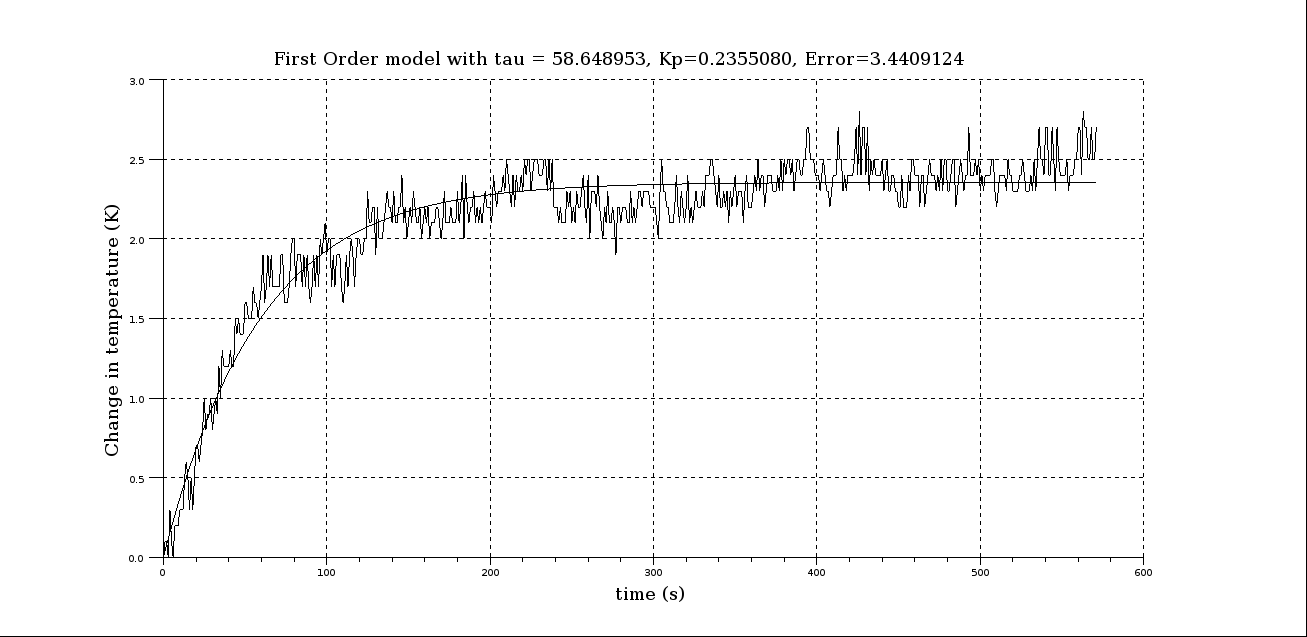
\includegraphics[width=\linewidth]{Step-test_manual/local-1-order.png}
\caption{Output of the Scilab code {\tt firstorder.sc}e for data file {\tt step-data-local.txt}}
\label{firstorder_output}
\end{figure} \label{firstorderplot}

\begin{align}
\intertext{The results presented are obtained for the data file {\tt step-data-virtual.txt}. This data file is present under the {\tt Step\_Test} directory for local experiments.The plot thus obtained is reasonably good. See the Scilab plot to get the values of $\tau$ and $K$. 
The figure \ref{firstorder_output} shows a screen shot of the same. We obtain $\tau$ = 58.64, K = 0.23. The transfer function 
obtained here is at the operating point of 30 percentage of heat. If the experiment is repeated at a different operating point, 
the transfer function obtained will be different. The gain will correspondingly be more at a higher operating point. 
This means that the plant is faster at higher temperature. Thus the transfer function of the plant varies with the operating 
point. Let the transfer function we obtain in this experiment be denoted as $G_s$. We obtain}
G_s(s) =  \frac{0.23}{58.64s+1} \label{12}
\end{align}
% \begin{figure}
% \centering
% 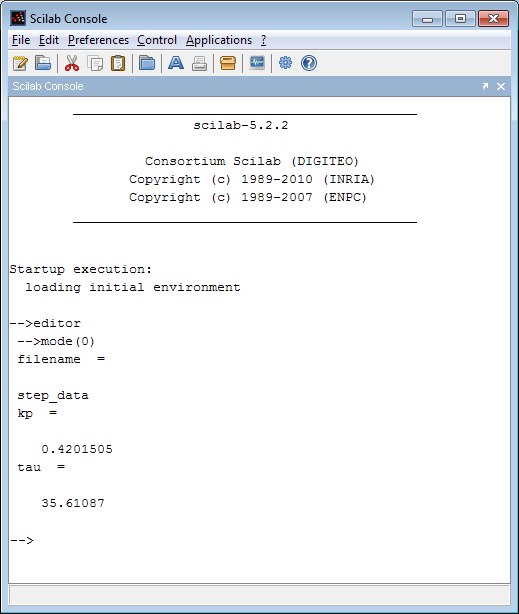
\includegraphics[width=\linewidth]{Step-test_manual/forder_console.png}
% \caption{The value of time constant and gain as shown on the console by \ttfamily firstorder.sce}
% \label{console}
% \end{figure}


\section{Determination of Second Order Transfer Function}
In this section, we explore the efficacy of a second order model of the form
\begin{align}
G(s) & = \frac K{(\tau_1s+1)(\tau_2s+1)} \label{eq:step-1100} 
\intertext{The response of the system to a step input of height $\Delta u$ is given by}
y(s) & = \frac K{(\tau_1s+1)(\tau_2s+1)} \frac{\Delta u}s 
\label{eq:step-1200} 
\end{align}

Splitting into partial fraction expansion, we obtain
\begin{align*}
y(s) & = \frac K{\tau_1\tau_2} \frac 1
{\left(s+\dfrac 1{\tau_1}\right)\left(s+\dfrac 1{\tau_2}\right)} =
\frac A s + \frac B{s+\dfrac 1{\tau_1}} + \frac C{s+\dfrac 1{\tau_2}}
\intertext{Through Heaviside expansion method, we determine the coefficients:}
A & = K \\
B & = -\frac{K\tau_1}{\tau_1-\tau_2} \\
C & = \frac{K\tau_2}{\tau_1-\tau_2}
\end{align*}

On substitution and inversion, we obtain
\begin{align}
y(t) & = K\left[ 1 - \frac 1{\tau_1-\tau_2}
\left( \tau_1 e^{-t/\tau_1} - \tau_2 e^{-t/\tau_2} \right)
\right] \label{eq:step-1300}
\end{align}

We have to determine three parameters $K$, $\tau_1$ and $\tau_2$
through optimization. Once again, we follow a procedure identical to the first order model.  
The only difference is that we now have to determine three parameters. Scilab code \\{\tt secondorder.sce} calculates
the gain and two time constants. 
\subsection {Procedure}
\begin{enumerate}
\item Download the Analysis folder from the sbhs website. It will be available under {\tt downloads} section. Download the file for {\tt SBHS Analysis Code (local \& virtual)}. The name of the file is {\tt scilab\_codes\_analysis}. The download will be in zip format. Extrat the downloaded zip file. You will get a folder {\tt scilab\_codes\_analysis}. 
\item Open the {\tt scilab\_codes\_analysis} folder and then locate and open the folder {\tt Step\_Analysis}.
\item Open the {\tt Kp-tau-order2} folder.
 \item Copy the step test data file to the folder {\tt Kp-tau-order2}.
 \item Change the Scilab working directory to {\tt Kp-tau-order2} folder under {\tt Step\_Analysis} folder.
 \item Open the file {\ttfamily secondorder.sce} in scilab editor and enter the name of the data file (with extention) in the {\tt filename} field. 
\item Save and run this code and obtain the plot as shown in figure \ref{sorder}. 
\end{enumerate}
\begin{align}
G_{s}(s) & = \frac {0.235}{(57.39s+1)(1s+1)}
\label{eq:step-1400}
\end{align}

\begin{figure}
\centering
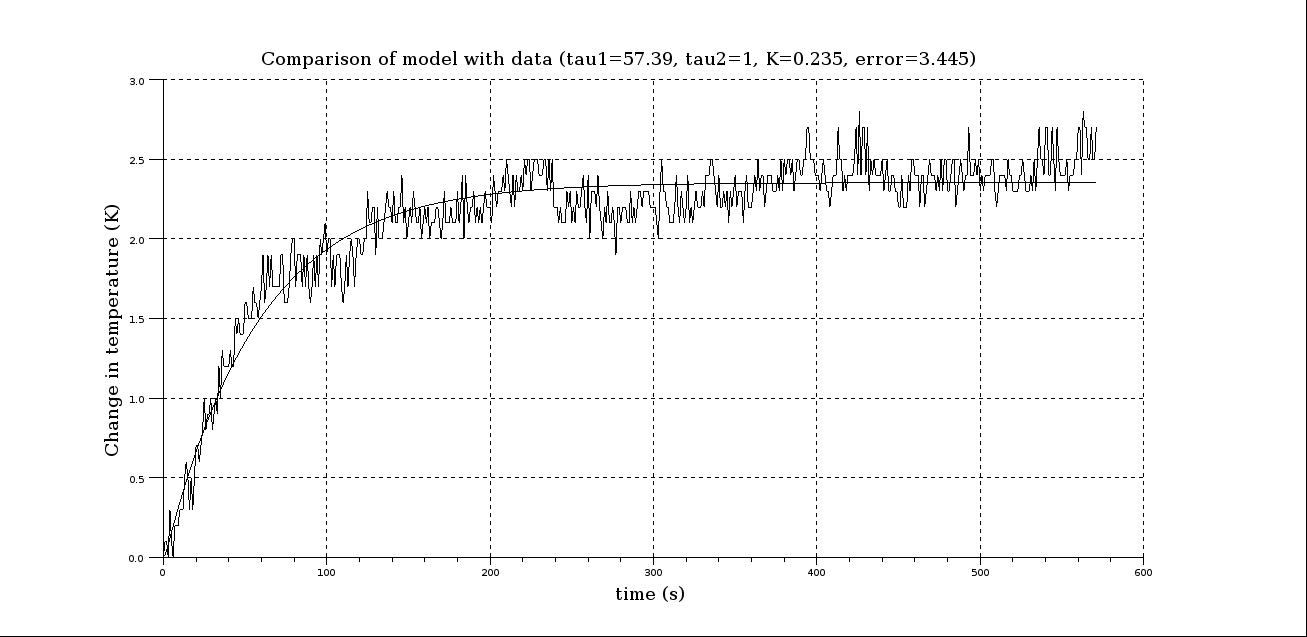
\includegraphics[width=\linewidth]{Step-test_manual/local-2-order.png}
\caption{Output of the Scilab code \ttfamily secondorder.sce}
\label{sorder}
\end{figure}

The fit is much better now.  In particular, the initial inflexion is well captured by this second
order transfer function.


\section{Discussion}
We summarize our findings now. For the first order analysis, the gain is 0.23 and the 
time constant $\tau$ is 58.64 seconds. For the second order analysis, the initial inflexion is 
well captured with the two time constants $\tau_1$=57.39, $\tau_2$= 1 and gain = 0.235. Negative steps 
can also be introduced to make the experiment more informative. One need not keep a particular 
input constant. By varying both the inputs, one can imagine it to be like a step varying disturbance signal.
 



\section{Scilab Code}\label{stepcodes}
\begin{code}
\ccaption{label.sci}{\ttfamily label.sci}
\lstinputlisting{Scilab/Analysis/Step_Analysis/Kp-tau-order1/label.sci}
\end{code}

\begin{code}
\ccaption{costf\_1.sci}{\ttfamily costf\_1.sci}
\lstinputlisting{Scilab/Analysis/Step_Analysis/Kp-tau-order1/costf_1.sci}
\end{code}


\begin{code}
\ccaption{firstorder.sce}{\ttfamily firstorder.sce}
\lstinputlisting{Scilab/Analysis/Step_Analysis/Kp-tau-order1/firstorder.sce}
\end{code}

\begin{code}
\ccaption{costf\_2.sci}{\ttfamily costf\_2.sci}
\lstinputlisting{Scilab/Analysis/Step_Analysis/Kp-tau-order2/costf_2.sci}
\end{code}

\begin{code}
\ccaption{order\_2\_heater.sci}{\ttfamily order\_2\_heater.sci}
\lstinputlisting{Scilab/Analysis/Step_Analysis/Kp-tau-order2/order_2_heater.sci}
\end{code}

\begin{code}
\ccaption{secondorder.sce}{\ttfamily secondorder.sce}
\lstinputlisting{Scilab/Analysis/Step_Analysis/Kp-tau-order2/secondorder.sce}
\end{code}

\begin{code}
\ccaption{ser\_init.sce}{\ttfamily ser\_init.sce}
\lstinputlisting{Scilab/local/Step_test/ser_init.sce}
\end{code}

\begin{code}
\ccaption{step\_test.sci}{\ttfamily step\_test.sci}
\lstinputlisting{Scilab/local/Step_test/step_test.sci}
\end{code}

\begin{code}
\ccaption{stepc.sce}{\ttfamily stepc.sce}
\lstinputlisting{Scilab/virtual/StepTest/stepc.sce}
\end{code}

\begin{code}
\ccaption{steptest.sci}{\ttfamily steptest.sci}
\lstinputlisting{Scilab/virtual/StepTest/steptest.sci}
\end{code}













